\documentclass[a4paper,12pt]{article}

\usepackage[spanish]{babel}
\usepackage[utf8]{inputenc}
\usepackage[T1]{fontenc}

%% Sets page size and margins
\usepackage[a4paper,margin=1in,marginparwidth=1in]{geometry}

%% Useful packages
\usepackage{amsmath}
\usepackage{breqn}
\usepackage{graphicx}
\usepackage[colorinlistoftodos]{todonotes}
\usepackage[colorlinks=true, allcolors=blue]{hyperref}
\usepackage{caption}
\usepackage{subcaption}
\usepackage{sectsty}
\usepackage{float}
\usepackage{titling} 
\usepackage{blindtext}
\usepackage[colorinlistoftodos]{todonotes}
\usepackage{xcolor}
\usepackage{textcomp}
\usepackage{hyperref}
\usepackage{fancyhdr}
\usepackage[style=ieee]{biblatex}
\usepackage{csquotes}
\usepackage{siunitx}
\usepackage{wrapfig}

\addbibresource{references.bib}
\definecolor{darkgreen}{rgb}{0.0, 0.4, 0.0}
\setlength{\headheight}{16pt}

\allowdisplaybreaks

\pagestyle{fancy}
\fancyhf{}
\rhead{Robótica}
\lhead{Manipulador \emph{{\textmu}Arm}}
\cfoot{\thepage}

%%%%%%%% DOCUMENT %%%%%%%%
\begin{document}

%%%% Title Page
\begin{titlepage}

    \newcommand{\HRule}{\rule{\linewidth}{0.5mm}}
    \center

    % University
    \textsc{\LARGE Universidad Politécnica de Madrid}\\[1cm]

    % Document info
    \textsc{\Large Robótica}\\[0.2cm]
    \textsc{\large \textit{MANIPULADORES}}\\[1cm]
    \HRule \\[0.8cm]
    { \huge \bfseries Estudio del manipulador \textit{{\textmu}Arm}}\\[0.7cm]
    \HRule \\[2cm]
    \large
    \emph{Autores:}\\
    Javier Alonso Silva - \href{mailto:javier.asilva@alumnos.upm.es}{javier.asilva@alumnos.upm.es}

    Roberto Álvarez Garrido - \href{mailto:roberto.alvarezg@alumnos.upm.es}{roberto.alvarezg@alumnos.upm.es}

    José Alejandro Moya Blanco - \href{mailto:alejandro.moya.blanco@alumnos.upm.es}{alejandro.moya.blanco@alumnos.upm.es}\\[1.5cm]
    {\large Última modificación: \today}\\[2cm]
    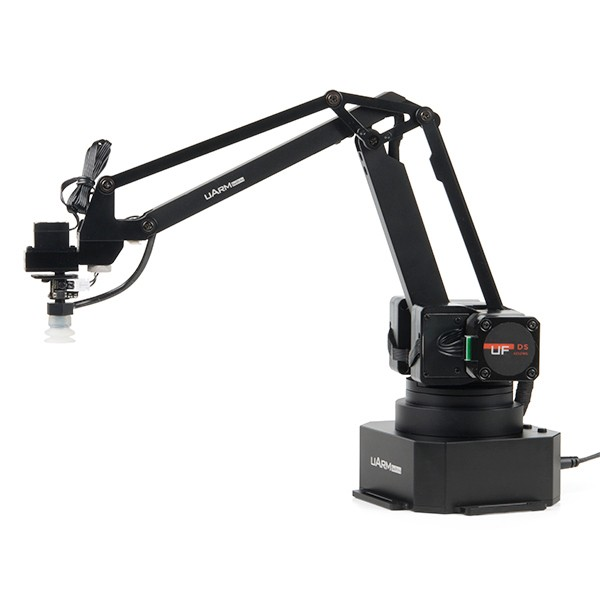
\includegraphics[width=0.5\textwidth]{images/uarm.jpg}\\[1cm]
\end{titlepage}

%%%% SECTIONS
\section*{Conocimientos previos}

Antes de ponernos a hablar sobre los resultados obtenidos en la práctica,
antes vamos a hablar sobre algunas características básicas del brazo robótico e
introducirlo brevemente.
El manipulador robótico \emph{{\textmu}Arm} es un dispositivo creado por la empresa
\href{https://www.ufactory.cc/#/}{UFACTORY} el cual cuenta con cuatro grados de libertad.
De dichos grados de libertad, tres son usados para mover el brazo robótico hasta ciertas
posiciones y, el último, para mantener el extremo del mismo paralelo al suelo.

\begin{wrapfigure}{R}{.4\textwidth}
    \begin{center}
        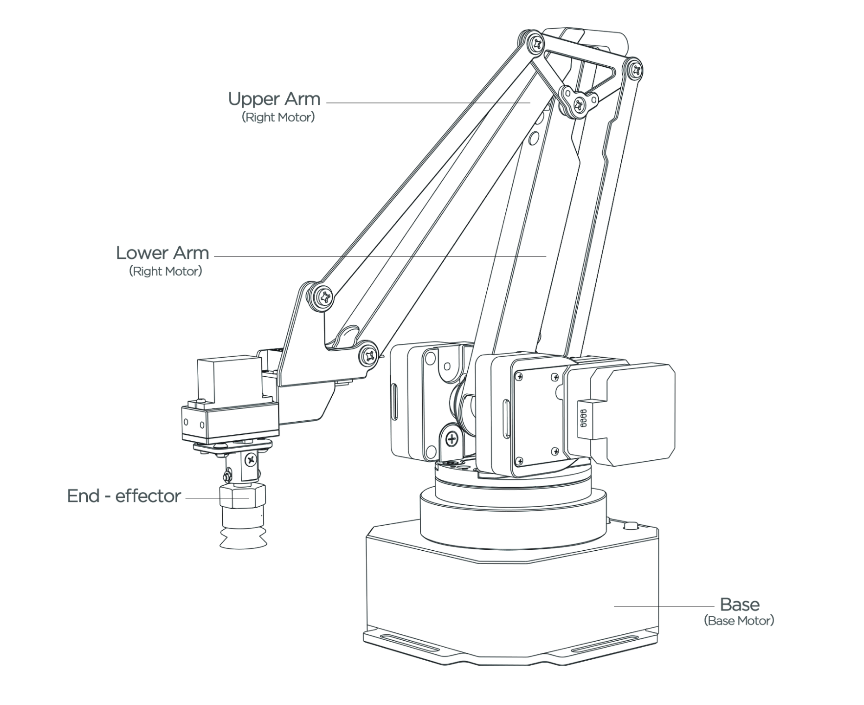
\includegraphics[width=.4\textwidth]{images/motors.png}
        \caption{zonas de actuación de los motores en el brazo \cite{developer_guide_uarm}}
        \label{fig:motors}
    \end{center}
\end{wrapfigure}

El manipulador es controlado mediante cuatro motores:

% \begin{itemize}
El \textbf{motor de la base} el cual permite la rotación del manipulador.

En el brazo, el \textbf{motor que está a la derecha} (ver la figura \ref{fig:motors}),
coordina el movimiento de la parte inferior del brazo (\textit{Lower Arm} en la figura)
con la parte superior del mismo (\textit{Upper Arm} en la figura).

En esta parte del manipulador, el movimiento es como el de un flexo: la parte superior
del flexo está supeditada a la parte inferior, de manera que se mantiene de forma
constante la altura a la que está el extremo final del mismo.

El otro motor, localizado a la \textbf{izquierda del brazo}, se encarga de mantener la
orientación del extremo del manipulador. De esta manera, dicho extremo
permanecerá paralelo al suelo. Teniendo en cuenta esto, podríamos decir
que el robot en verdad solo tiene tres grados de libertad en tanto a que no se
controla directamente el movimiento del último grado, ya que al final se mueve
para permanecer paralelo al suelo.

El \textbf{motor localizado en el extremo}, con el cual se puede actuar sobre el
elemento que esté colocado allí. Por ejemplo, cuando se coloca una ventosa
permite rotarla o, cuando se coloca la pinza, el movimiento del motor permite
abrirla o cerrarla.

Para este estudio, este último motor se descartará, ya que no afecta a las
posiciones accesibles por el robot.
% \end{itemize}

\begin{table}[ht]
    \begin{minipage}{.49\linewidth}
        \centering
        \begin{tabular}{||c | c||}
            \hline
            \textit{Motor} & \textit{Rango de trabajo} \\ [0.5ex]
            \hline\hline
            Base           & $\ang{0} \sim \ang{180}$  \\
            \hline
            Derecho        & $\ang{0} \sim \ang{130}$  \\
            \hline
            Izquierdo      & $\ang{0} \sim \ang{106}$  \\
            \hline
            Extremo        & $\ang{0} \sim \ang{180}$  \\ [1ex]
            \hline
        \end{tabular}
        \caption{ángulo de giro de los motores}
    \end{minipage}
    \hfill
    \begin{minipage}{.49\linewidth}
        \begin{figure}[H]
            \centering
            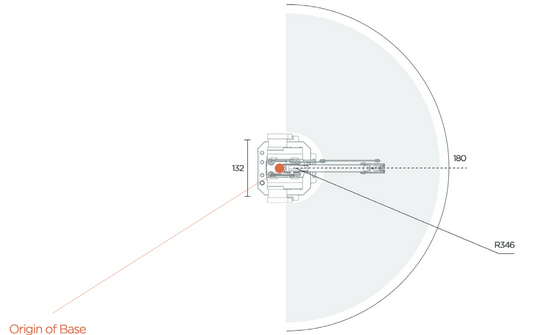
\includegraphics[width=\linewidth]{images/range.png}
            \caption{rango del manipulador \emph{{\textmu}Arm} \cite{user_manual_uarm}}
            \label{fig:range}
        \end{figure}
    \end{minipage}
\end{table}

\newpage
Toda la información relativa al desarrollo del proyecto puede ser encontrada en
\href{https://github.com/UPM-Robotics/uarm}{GitHub - UPM Robotics} \cite{noauthor_upm-robotics/uarm_2019}. Allí están detallados
los distintos hitos a conseguir así como más información sobre el robot.

Además, se encuentra disponible la siguiente bibliografía:
\begin{itemize}
    \item \href{https://github.com/UPM-Robotics/uarm/blob/master/docs/robot-information/uArm%20pro%20User%20Manual%20v1.1.0.pdf}{Manual de usuario}
    \item \href{https://github.com/UPM-Robotics/uarm/blob/master/docs/robot-information/uArm-Swift-Specifications-171012.pdf}{Especificaciones}
    \item \href{https://github.com/UPM-Robotics/uarm/blob/master/docs/robot-information/uArm%20Swift%20Pro_Developer%20Guide%20v1.0.6.pdf}{Guía del desarrollador}
    \item \href{https://github.com/UPM-Robotics/uarm/blob/master/docs/robot-information/uArm_Swift_Pro_3D_20180620.STEP}{Modelo en 3D}
    \item \href{https://www.ufactory.cc/#/en/}{Web de UFACTORY}
    \item \href{https://www.ufactory.cc/#/en/support/technology}{Soporte de UFACTORY}
\end{itemize}

\newpage
\section{Configuración geométrica}

En esta sección vamos a describir la configuración geométrica del brazo robótico. La
configuración que obtuvimos fue la siguiente:
\begin{figure}[H]
    \begin{minipage}{.4\linewidth}
        \centering
        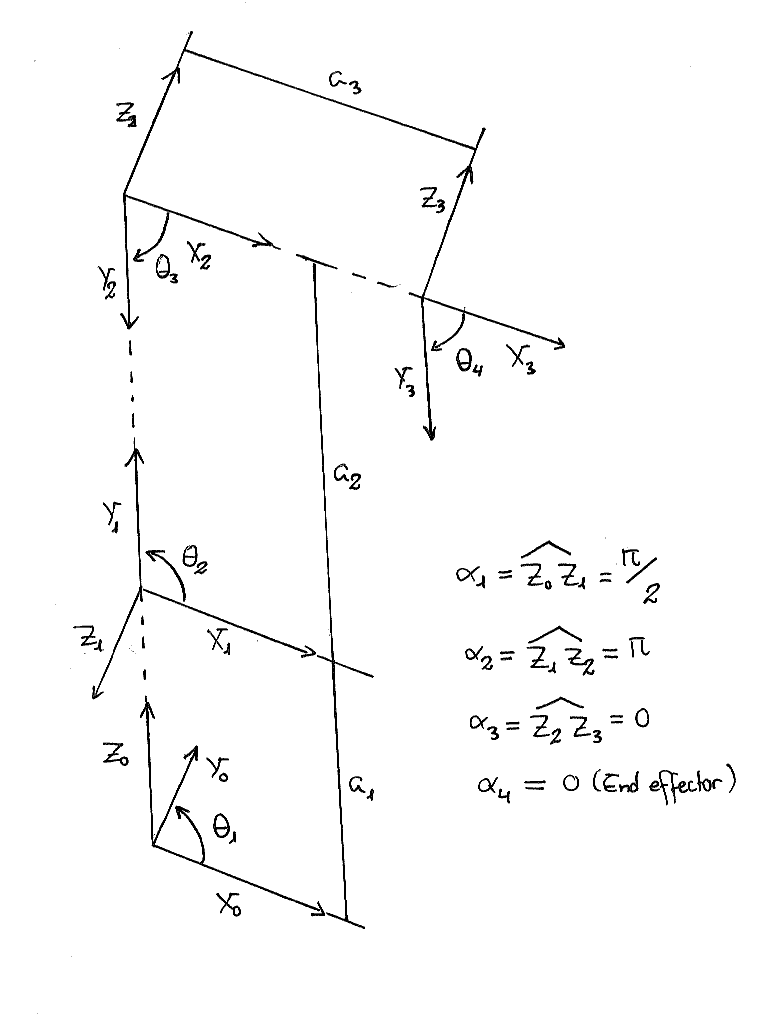
\includegraphics[width=\linewidth]{images/geometric_configuration_2.png}
        \caption{configuración geométrica del robot}
        \label{fig:robot_config}
    \end{minipage}\hfill
    \begin{minipage}{.48\linewidth}
        \centering
        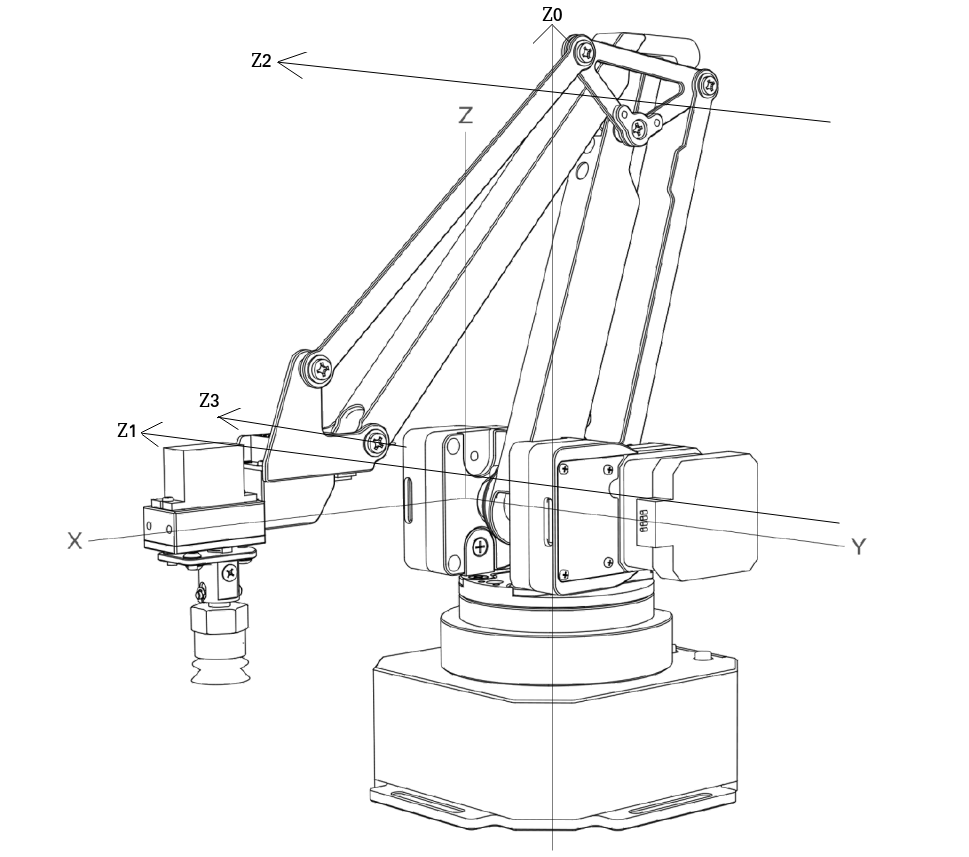
\includegraphics[width=\linewidth]{images/axis.png}
        \caption{los grados de libertar del brazo, representados por los diferentes $Z_i$}
        \label{fig:axis}
    \end{minipage}
\end{figure}

Usando los datos que están presentes en la documentación al desarrollador \cite{developer_guide_uarm},
pudimos obtener los siguientes datos para los $a_i$ (distancia entre ejes) del manipulador; además,
descubrimos que hay una pequeña desviación $d_i$ entre las articulaciones $\{1, 2\}$:

\begin{table}[ht]
    \begin{minipage}{.49\linewidth}
        \begin{figure}[H]
            \centering
            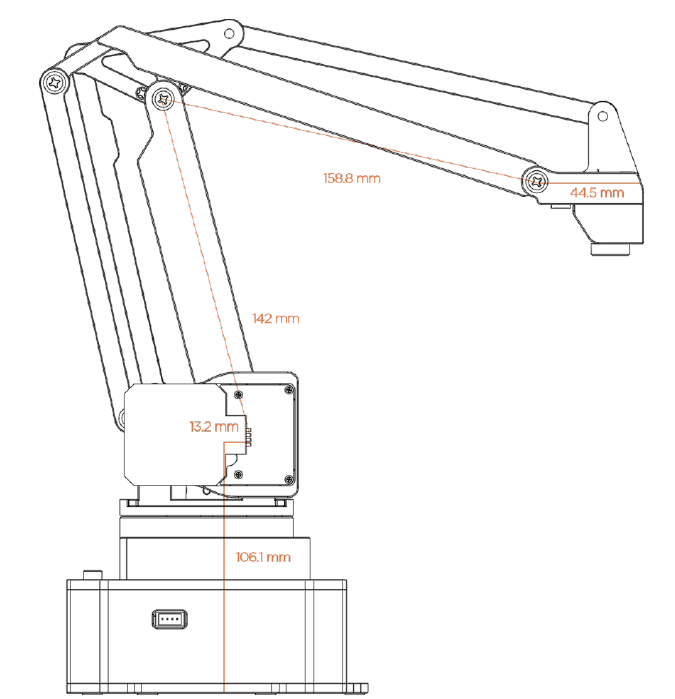
\includegraphics[width=\linewidth]{images/sizes.png}
            \caption{longitudes del brazo robótico \cite{developer_guide_uarm}}
            \label{fig:sizes}
        \end{figure}
    \end{minipage}
    \hfill
    \begin{minipage}{.49\linewidth}
        \centering
        \begin{tabular}{|| c | c c ||}
            \hline
            $i$ & $a_i~(mm.)$ & $d_i~(mm.)$ \\ [0.5ex]
            \hline\hline
            $1$ & $106.1$     & $13.2$      \\
            \hline
            $2$ & $142$       & $0$         \\
            \hline
            $3$ & $158.8$     & $0$         \\
            \hline
            $4$ & $44.5$      & $0$         \\ [1ex]
            \hline
        \end{tabular}
        \caption{longitudes y desviaciones del manipulador}
    \end{minipage}
\end{table}

De esta manera, con los datos obtenidos, generamos una primera matriz de \textit{Denavit-Hartenberg}:

\begin{table}[H]
    \parbox{.45\linewidth}{
        \centering
        \begin{tabular}{ c | c c c c }
            $i$ & $\theta_i$ & $d_i~(mm.)$ & $a_i~(mm.)$ & $\alpha_i$      \\ [0.5ex]
            \hline
            $1$ & $\theta_1$ & $13.2$      & $106.1$     & $\frac{\pi}{2}$ \\
            $2$ & $\theta_2$ & $0$         & $142$       & $\pi$           \\
            $3$ & $\theta_3$ & $0$         & $158.8$     & $0$             \\
            $4$ & $\theta_4$ & $0$         & $44.5$      & $0$             \\ [1ex]
        \end{tabular}
        \caption{primera tabla de \textit{Denavit–Hartenberg}}
    }
    \hfill
    \parbox{.45\linewidth}{
        \centering
        \begin{tabular}{ c | c c c c }
            $i$ & $\theta_i$ & $d_i~(mm.)$ & $a_i~(mm.)$ & $\alpha_i$      \\ [0.5ex]
            \hline
            $1$ & $\theta_1$ & $d_1$       & $a_1$       & $\frac{\pi}{2}$ \\
            $2$ & $\theta_2$ & $0$         & $a_2$       & $\pi$           \\
            $3$ & $\theta_3$ & $0$         & $a_3$       & $0$             \\
            $4$ & $\theta_4$ & $0$         & $a_4$       & $0$             \\ [1ex]
        \end{tabular}
        \caption{primera tabla de \textit{Denavit–Hartenberg} parametrizada}
    }
\end{table}

La cuestión es que, al hacer los distintos modelos, descubrimos que debido a la orientación del brazo
robótico, la $d_i$ está en la posición del equivalente $a_i$, en particular $d_1$ y $a_1$.
Esto es debido a que, como se puede ver en la figura \ref{fig:axis} junto con las figuras \ref{fig:robot_config}
y \ref{fig:sizes}, el plano sobre el que está $d_i$ es el $XZ$, lo cual nos obliga a cambiar las posiciones
en las que existen a la vez un $a_i$ y un $d_i$, siempre y cuando ambos sean constantes, que en este caso lo son.
De esta forma, la tabla de \textit{Denavit-Hartenberg} quedaría:

\begin{table}[H]
    \parbox{.45\linewidth}{
        \centering
        \begin{tabular}{ c | c c c c }
            $i$ & $\theta_i$ & $d_i~(mm.)$ & $a_i~(mm.)$ & $\alpha_i$      \\ [0.5ex]
            \hline
            $1$ & $\theta_1$ & $106.1$     & $13.2$      & $\frac{\pi}{2}$ \\
            $2$ & $\theta_2$ & $0$         & $142$       & $\pi$           \\
            $3$ & $\theta_3$ & $0$         & $158.8$     & $0$             \\
            $4$ & $\theta_4$ & $0$         & $44.5$      & $0$             \\ [1ex]
        \end{tabular}
        \caption{segunda tabla de \textit{Denavit–Hartenberg}}
    }
    \hfill
    \parbox{.45\linewidth}{
        \centering
        \begin{tabular}{ c | c c c c }
            $i$ & $\theta_i$ & $d_i~(mm.)$ & $a_i~(mm.)$ & $\alpha_i$      \\ [0.5ex]
            \hline
            $1$ & $\theta_1$ & $a_1$       & $d_1$       & $\frac{\pi}{2}$ \\
            $2$ & $\theta_2$ & $0$         & $a_2$       & $\pi$           \\
            $3$ & $\theta_3$ & $0$         & $a_3$       & $0$             \\
            $4$ & $\theta_4$ & $0$         & $a_4$       & $0$             \\ [1ex]
        \end{tabular}
        \caption{segunda tabla de \textit{Denavit–Hartenberg} parametrizada}
    }
\end{table}

Finalmente, el \textit{end-effector} (véase la figura \ref{fig:motors}) siempre está perpendicular
al plano del suelo, es decir, $\phi_e = \pi$. Por eso mismo, el parámetro $i = 4$ en verdad
está supeditado siempre al movimiento que se realice según los ángulos $\theta_2$ y $\theta_3$, así
que no es necesario contemplarlo en la tabla de \textit{Denavit-Hartenberg}:

\begin{table}[H]
    \parbox{.45\linewidth}{
        \centering
        \begin{tabular}{ c | c c c c }
            $i$ & $\theta_i$ & $d_i~(mm.)$ & $a_i~(mm.)$ & $\alpha_i$      \\ [0.5ex]
            \hline
            $1$ & $\theta_1$ & $106.1$     & $13.2$      & $\frac{\pi}{2}$ \\
            $2$ & $\theta_2$ & $0$         & $142$       & $\pi$           \\
            $3$ & $\theta_3$ & $0$         & $158.8$     & $0$             \\ [1ex]
        \end{tabular}
        \caption{tabla de \textit{Denavit–Hartenberg}}
    }
    \hfill
    \parbox{.45\linewidth}{
        \centering
        \begin{tabular}{ c | c c c c }
            $i$ & $\theta_i$ & $d_i~(mm.)$ & $a_i~(mm.)$ & $\alpha_i$      \\ [0.5ex]
            \hline
            $1$ & $\theta_1$ & $a_1$       & $d_1$       & $\frac{\pi}{2}$ \\
            $2$ & $\theta_2$ & $0$         & $a_2$       & $\pi$           \\
            $3$ & $\theta_3$ & $0$         & $a_3$       & $0$             \\ [1ex]
        \end{tabular}
        \caption{tabla de \textit{Denavit–Hartenberg} parametrizada}
    }
\end{table}

\section{Cinemática directa}
A continuación, con los valores obtenidos en el apartado anterior, vamos a obtener las
distintas matrices de transformación de referenciales de manipuladores. Para ello, partimos de la
siguiente matriz:

\[
    A_{i-1}^i =
    \begin{pmatrix}
        \cos\theta_i & -\cos\alpha_i\sin\theta_i & \sin\alpha_i\sin\theta_i  & a_i\cos\theta_i \\
        \sin\theta_i & \cos\alpha_i\cos\theta_i  & -\sin\alpha_i\cos\theta_i & a_i\sin\theta_i \\
        0            & \sin\alpha_i              & \cos\alpha_i              & d_i             \\
        0            & 0                         & 0                         & 1
    \end{pmatrix}
\]

Aplicando los distintos pasos, obtenemos:

\begin{align*}
    A_0^1 &=
    \begin{pmatrix}
        \cos{\left(\theta_{1} \right)} & 0 & \sin{\left(\theta_{1} \right)}   & d_{1} \cos{\left(\theta_{1} \right)} \\
        \sin{\left(\theta_{1} \right)} & 0 & - \cos{\left(\theta_{1} \right)} & d_{1} \sin{\left(\theta_{1} \right)} \\
        0                              & 1 & 0                                & a_{1}                                \\
        0                              & 0 & 0                                & 1                                    \\
    \end{pmatrix} \\
    A_1^2 &=
    \begin{pmatrix}
        \cos{\left(\theta_{2} \right)} & \sin{\left(\theta_{2} \right)}   & 0  & a_{2} \cos{\left(\theta_{2} \right)} \\
        \sin{\left(\theta_{2} \right)} & - \cos{\left(\theta_{2} \right)} & 0  & a_{2} \sin{\left(\theta_{2} \right)} \\
        0                              & 0                                & -1 & 0                                    \\
        0                              & 0                                & 0  & 1                                    \\
    \end{pmatrix} \\
    A_2^3 &=
    \begin{pmatrix}
        \cos{\left(\theta_{3} \right)} & - \sin{\left(\theta_{3} \right)} & 0 & a_{3} \cos{\left(\theta_{3} \right)} \\
        \sin{\left(\theta_{3} \right)} & \cos{\left(\theta_{3} \right)}   & 0 & a_{3} \sin{\left(\theta_{3} \right)} \\
        0                              & 0                                & 1 & 0                                    \\
        0                              & 0                                & 0 & 1                                    \\
    \end{pmatrix}
\end{align*}

Con todas las matrices ya obtenidas, podemos calcular la matriz de
transformación directa del manipulador (son 4 columnas, pero no cabe la matriz al completo, por eso la última columna está debajo):

{\footnotesize\begin{align*}
    A_0^2 &=
    \begin{pmatrix}
        \cos{\left(\theta_{1} \right)} \cos{\left(\theta_{2} \right)} & \sin{\left(\theta_{2} \right)} \cos{\left(\theta_{1} \right)} & - \sin{\left(\theta_{1} \right)} & \left(a_{2} \cos{\left(\theta_{2} \right)} + d_{1}\right) \cos{\left(\theta_{1} \right)} \\
        \sin{\left(\theta_{1} \right)} \cos{\left(\theta_{2} \right)} & \sin{\left(\theta_{1} \right)} \sin{\left(\theta_{2} \right)} & \cos{\left(\theta_{1} \right)}   & \left(a_{2} \cos{\left(\theta_{2} \right)} + d_{1}\right) \sin{\left(\theta_{1} \right)} \\
        \sin{\left(\theta_{2} \right)}                                & - \cos{\left(\theta_{2} \right)}                              & 0                                & a_{1} + a_{2} \sin{\left(\theta_{2} \right)}                                             \\
        0                                                             & 0                                                             & 0                                & 1                                                                                        \\
    \end{pmatrix} \\
    A_0^3 &=
    \begin{pmatrix}
        \cos{\left(\theta_{1} \right)} \cos{\left(\theta_{2} - \theta_{3} \right)} & \sin{\left(\theta_{2} - \theta_{3} \right)} \cos{\left(\theta_{1} \right)}                                                                          & - \sin{\left(\theta_{1} \right)} \\
        \sin{\left(\theta_{1} \right)} \cos{\left(\theta_{2} - \theta_{3} \right)} & \sin{\left(\theta_{1} \right)} \sin{\left(\theta_{2} - \theta_{3} \right)}                                                                          & \cos{\left(\theta_{1} \right)}   \\
        \sin{\left(\theta_{2} - \theta_{3} \right)}                                & - \cos{\left(\theta_{2} - \theta_{3} \right)}                                                                                                       & 0                                \\
        0                                                                          & 0                                                                                                                                                   & 0                                \\
                                                                                   & \qquad \left(a_{2} \cos{\left(\theta_{2} \right)} + a_{3} \cos{\left(\theta_{2} - \theta_{3} \right)} + d_{1}\right) \cos{\left(\theta_{1} \right)}                                    \\
                                                                                   & \qquad \left(a_{2} \cos{\left(\theta_{2} \right)} + a_{3} \cos{\left(\theta_{2} - \theta_{3} \right)} + d_{1}\right) \sin{\left(\theta_{1} \right)}                                    \\
                                                                                   & \qquad a_{1} + a_{2} \sin{\left(\theta_{2} \right)} + a_{3} \sin{\left(\theta_{2} - \theta_{3} \right)}                                                                                \\
                                                                                   & \qquad 1
    \end{pmatrix}
\end{align*}}

Las matrices están parametrizadas. Numéricamente, la matriz de transformación directa $A_0^3$ quedaría:

{\footnotesize\begin{align*}
    A_0^3 &=
    \begin{pmatrix}
        \cos{\left(\theta_{1} \right)} \cos{\left(\theta_{2} - \theta_{3} \right)} & \sin{\left(\theta_{2} - \theta_{3} \right)} \cos{\left(\theta_{1} \right)}                                                                         & - \sin{\left(\theta_{1} \right)} \\
        \sin{\left(\theta_{1} \right)} \cos{\left(\theta_{2} - \theta_{3} \right)} & \sin{\left(\theta_{1} \right)} \sin{\left(\theta_{2} - \theta_{3} \right)}                                                                         & \cos{\left(\theta_{1} \right)}   \\
        \sin{\left(\theta_{2} - \theta_{3} \right)}                                & - \cos{\left(\theta_{2} - \theta_{3} \right)}                                                                                                      & 0                                \\
        0                                                                          & 0                                                                                                                                                  & 0                                \\
                                                                                   & \qquad \left(142.0 \cos{\left(\theta_{2} \right)} + 158.9 \cos{\left(\theta_{2} - \theta_{3} \right)} + 13.2\right) \cos{\left(\theta_{1} \right)}                                    \\
                                                                                   & \qquad \left(142.0 \cos{\left(\theta_{2} \right)} + 158.9 \cos{\left(\theta_{2} - \theta_{3} \right)} + 13.2\right) \sin{\left(\theta_{1} \right)}                                    \\
                                                                                   & \qquad 142.0 \sin{\left(\theta_{2} \right)} + 158.9 \sin{\left(\theta_{2} - \theta_{3} \right)} + 106.1                                                                               \\
                                                                                   & \qquad 1                                                                                                                                                                              \\
    \end{pmatrix}
\end{align*}}

Finalmente, hay que añadir una traslación en el eje $Z$ (debido a la posición del \textit{end-effector})
y en el eje $X$, ya que después de la articulación $\theta_3$ hay una extensión de $44,5~mm.$ (ver figura \ref{fig:sizes}),
para obtener así la posición final del robot $(X_e ~ Y_e ~ Z_e)$:

{\footnotesize\begin{align*}
    A_0^3 &=
    \begin{pmatrix}
        \cos{\left(\theta_{1} \right)} \cos{\left(\theta_{2} - \theta_{3} \right)} & \sin{\left(\theta_{2} - \theta_{3} \right)} \cos{\left(\theta_{1} \right)}                                                                          & - \sin{\left(\theta_{1} \right)} \\
        \sin{\left(\theta_{1} \right)} \cos{\left(\theta_{2} - \theta_{3} \right)} & \sin{\left(\theta_{1} \right)} \sin{\left(\theta_{2} - \theta_{3} \right)}                                                                          & \cos{\left(\theta_{1} \right)}   \\
        \sin{\left(\theta_{2} - \theta_{3} \right)}                                & - \cos{\left(\theta_{2} - \theta_{3} \right)}                                                                                                       & 0                                \\
        0                                                                          & 0                                                                                                                                                   & 0                                \\
                                                                                   & \qquad \left(a_{2} \cos{\left(\theta_{2} \right)} + a_{3} \cos{\left(\theta_{2} - \theta_{3} \right)} + d_{1}\right) \cos{\left(\theta_{1} \right)} + T_X                                   \\
                                                                                   & \qquad \left(a_{2} \cos{\left(\theta_{2} \right)} + a_{3} \cos{\left(\theta_{2} - \theta_{3} \right)} + d_{1}\right) \sin{\left(\theta_{1} \right)}                                    \\
                                                                                   & \qquad a_{1} + a_{2} \sin{\left(\theta_{2} \right)} + a_{3} \sin{\left(\theta_{2} - \theta_{3} \right)} - T_{Z}                                                                                \\
                                                                                   & \qquad 1
    \end{pmatrix} \\
    A_0^3 &=
    \begin{pmatrix}
        \cos{\left(\theta_{1} \right)} \cos{\left(\theta_{2} - \theta_{3} \right)} & \sin{\left(\theta_{2} - \theta_{3} \right)} \cos{\left(\theta_{1} \right)}                                                                         & - \sin{\left(\theta_{1} \right)} \\
        \sin{\left(\theta_{1} \right)} \cos{\left(\theta_{2} - \theta_{3} \right)} & \sin{\left(\theta_{1} \right)} \sin{\left(\theta_{2} - \theta_{3} \right)}                                                                         & \cos{\left(\theta_{1} \right)}   \\
        \sin{\left(\theta_{2} - \theta_{3} \right)}                                & - \cos{\left(\theta_{2} - \theta_{3} \right)}                                                                                                      & 0                                \\
        0                                                                          & 0                                                                                                                                                  & 0                                \\
                                                                                   & \left(142.0 \cos{\left(\theta_{2} \right)} + 158.9 \cos{\left(\theta_{2} - \theta_{3} \right)} + 13.2\right) \cos{\left(\theta_{1} \right)} + 44,5                                   \\
                                                                                   & \left(142.0 \cos{\left(\theta_{2} \right)} + 158.9 \cos{\left(\theta_{2} - \theta_{3} \right)} + 13.2\right) \sin{\left(\theta_{1} \right)}                                    \\
                                                                                   & 142.0 \sin{\left(\theta_{2} \right)} + 158.9 \sin{\left(\theta_{2} - \theta_{3} \right)} + 106,1 - T_Z                                                                              \\
                                                                                   & 1                                                                                                                                                                              \\
    \end{pmatrix}
\end{align*}}

\newpage
\printbibliography

\end{document}